\documentclass[11pt,a4paper]{scrartcl}
\usepackage[latin1]{inputenc}
\usepackage{amsmath}
\usepackage{amsfonts}
\usepackage{amssymb}
\usepackage{graphicx}
\usepackage{longtable}
\usepackage{array}

\usepackage{listings}
\usepackage{tikz}
\tikzset{main node/.style={circle,fill=blue!20,draw,minimum size=1cm,inner sep=0pt},
}

\addtokomafont{disposition}{\rmfamily}



\title{MSc, MEng and MMath Examinations, 2017?18
	DEPARTMENT OF COMPUTER SCIENCE
	Model-Driven Engineering (MODE)
	Open Individual Assessment}
\date{}

\begin{document}
	%-----------------------------------------------------
	% Title Page
	%-----------------------------------------------------
	
	\begin{titlepage}
		\begin{center}
			
			\large
			\textbf{University of York} \\
			\vspace{0.2cm}
			\textbf{MSc, MEng and MMath Examinations, 2017-18} \\
			\vspace{0.2cm}
			\textbf{DEPARTMENT OF COMPUTER SCIENCE} \\
			
			\vspace{2cm}
			
			\huge
			\textbf{Model-Driven Engineering (MODE)} 
			\textbf{Open Individual Assessment} \\
			
			\vspace{2cm}
			
			\Large
			\textbf{Examination Number} \\
			\textbf{Y1403115}
			
		\end{center}
	\end{titlepage}
	
	


\section{Abstract Syntax and Constraints}
%Explain how you have arrived at the abstract
%syntax and any well-formedness constraints for your DSL, justify the decisions
%that you have made, and discuss how you have tested your abstract syntax and
%well-formedness constraints.

	\subsection{Problem analysis}
	A domain specific language(DSL) needs to be created which allows the creation, modification and modelling relationships between four entities - system requirements, customer requirements, team members and test cases. Possible relationships between two requirements can be decomposition(also referred to as dependency in this report) and conflict. Requirements can be assigned to team members and can also be verified by test cases. 
	The implementation of the metamodel in Emfatic defines 4 concrete classes for each of the entities mentioned above along with a container class RequirementsModel and a few abstract classes defined to limit duplication and enforce constraints.
	
	\begin{lstlisting}
	class RequirementsModel
	abstract class Identifiable
	abstract class Describable
	abstract class Requirement extends Identifiable, Describable
	class CustomerRequirement extends Requirement
	class SystemRequirement extends Requirement
	class TestCase extends Identifiable, Describable
	class TeamMember extends Identifiable
	\end{lstlisting}
	
	\subsection{Abstract classes}
	System requirements and customer requirements share a number of common properties. It is obvious that having a super class Requirement, which captures these common properties is beneficial and avoids duplication. All requirements have a progress attribute and an updateProgress operation which will be discussed later on.
	
	According to the specification, both requirements and test-cases need to have a description. This is a string attribute in terms of the Emfatic code. In order to avoid duplication by defining this attribute in both classes an abstract class Describable is used, which is a superclass of both requirements and test-cases.
	
	Requirements also must have an unique identifier. While not specifically stated in the specification, being able to uniquely identify test-cases and team members is an important property of the DSL, as it avoids visual ambiguity for users, maintaining models. For this reason the abstract class Identifiable is defined, which has a string attribute id, and is a super class of requirements, test-cases and team members.
	
	\subsection{Requirements Relationships}
	Requirements are the most important entities in the DSL. They form a directed acyclic graph structure of decomposition relationships. For simplicity a parent-child abstraction is used to model this relationship. That is requirements being decomposed are parents of requirements in the decomposition and the latter are children of the former. The decomposition relationships can be viewed as breaking down requirements into multiple smaller child requirements, which together form the parent requirement. This must be true because, according to the specification, parent requirement's progress is the average of it's children, which is 100\% when all of it's children are also 100\%. Further constraints on this realationship are:
	
	\begin{enumerate}
		\item Customer requirements can be decomposed into technical requirements, but not the other way round.
		\item Each customer requirement needs to be decomposed into at least one technical requirement.
		\item Each technical requirement needs originate from at least one customer requirement.
	\end{enumerate}
	
	This means that the graph of requirements must have 
	
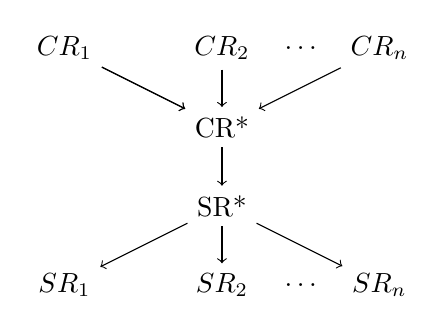
\begin{tikzpicture}

	\node (a) at (0,3)  {$CR_1$};
	\node (b) at (2,3)  {$CR_2$};
	\node (c) at (3,3)  {$\ldots$};
	\node (d) at (4,3)  {$CR_n$};
	
	\node (e) at (2,2)  {CR*};
	
	\node (f) at (2,1)  {SR*};
	
	\node (g) at (0,0)  {$SR_1$};
	\node (h) at (2,0)  {$SR_2$};
	\node (i) at (3,0)  {$\ldots$};
	\node (j) at (4,0)  {$SR_n$};
	
	\draw (a) edge[->] (e) 
	(a) edge[->] (e)
	(b) edge[->] (e)
	(d) edge[->] (e)
	(e) edge[->] (f)
	(f) edge[->] (g)
	(f) edge[->] (h)
	(f) edge[->] (j);
	
\end{tikzpicture}
	
	\pagebreak
	The problem is to construct a domain-specific language (DSL) for requirements modelling, which supports requirements (system and customer), team members and test cases. This means that the meta model, the DSL conforms to, should define EClasses for system and customer requirements, team members and test cases, as well as an abstract class for general requirements (given that they share some properties). In addition there needs to be a top level class, which contains all the entities, in order to comply with the tools that are used. 
	
	The assessment brief specifies several requirements for the DSL, from which several derived requirements can be defined. In this section of the report the interpretation of the problem will be discussed. 

	\subsection{Identifier and description}
	The assessment directly specifies that requirements and test cases need to have a description. In order to avoid duplication it is sensible to create an abstract class Describable which has a description attribute and they both extend.
	
	Requirements also need to have an identifier attribute, which is unique. Altough not explicitly specified this attribute is useful for both test cases and team members, since it makes them distinguishable by the user. For this reason an abstract class Identifiable is defined which has an attribute id and requirements, test cases and team members all extend it.
	
	\begin{enumerate}
		\item Each requirement has an identifier and a textual description.
		\item Each test-case has a description.
	\end{enumerate}
	


	\subsection{Requirements}
	Requirements can be one of two types - system and customer. In the metamodel Requirements is an abstract superclass with subclasses SystemRequirement and CustomerRequirement. All requirements have an integer progress attribute, which defaults to 0. Two main features of requirements are dpendencies(decomposition) amd conflicts, which are discussed in the following: 
	
	\subsection{Dependencies}
	Requirements are part of a tree-like structure where each requirement can be decomposed into several child requirements. Additional constraints, which come directly from the assessment, on this decomposition are that system requirements cannot be decomposed into customer requirements, customer requirements need to have at least one system requirement descendant and system requirements need to have at least one ancestor. This means that the requirement tree has only customer requirements at the top followed by system requirements at the bottom.
	
	To model this relationship in the meta model the Requirements superclass has a multivalued reference of type Requirement, for both the children and parents of the requirement. The additional constraints are handled by the model validation constraints. An alternative solution is to have the children and parent references in the subclasses like so
	
	\begin{lstlisting}
class CustomerRequirement extends Requirement{
	ref Requirement[*]#conflictsIncoming customerChildren;
	ref CustomerRequirement[*] customerParents;
}

class SystemRequirement extends Requirement{
	ref SystemRequirement[*]#systemParents systemChildren;
	ref Requirement[*] systemParents;
}
	\end{lstlisting}
	
	This way system requirements are restricted to have only system requirements as children. However an opposite for systemParents has to be both customerChildren and systemChildren, which is not possible in Ecore and being able to navigate from children to parents as well as the other way around is very important for the model management tasks.
	
	\subsection{Conflicts}
	The restriction on conflicts is that C
	
	\subsection{Test Cases}
	
	\subsection{Team Members}
	
	\subsection{Constraints}


\section{Editor}
%Explain the editor for your DSL, justify the decisions that you have made,
%and briefly argue why your editor provides an appropriate notation for your DSL.


\section{Model Management Operations}
%Explain the model management operations for
%your DSL, justify the decisions that you have made, and briefly demonstrate that
%the model management operations can be used to fulfill the model management
%tasks described in Section 1.	

	
\end{document}
